\section{Intro}
Most progress items can be categorized into the following three groups:
\begin{itemize}
    \item Establishing CLAS12 SubMIT at MIT
    \item Improving Monitoring, Documentation, and Code Fidelity
    \item Multitude of Small Code Improvements
\end{itemize}

\section{Establishing CLAS12 SubMIT at MIT}
    The CLAS12 system needs to be re-setup on MIT's Tier 2 systems (it was installed in 2019 but is now out of date and needs some touch ups). After this, it needs to be integrated to be accessible by CLAS12's webportal. 
    \subsection{Establish CLAS12 Simulations on MIT's Systems}
        We need to be able to submit jobs manually to HTCondor on tier 2 using SQLite testing databases. Currently the intfrastructure exists but the code is broken.
    \subsection{Resolve Python versioning issues}
        Python 2.6.6 is on submit.mit.edu this needs to be updated – no longer supported! Ended in 2013
        Python 2 support ended in 2020, so we really need python3
        Actually, also there is python 2.7.6 on SubMIT but there seems to be some module issue with SQLite:
        
        
        \begin{lstlisting}
            -bash-4.1$ python2.7 create_database.py --lite=clas12ocr.db     
            Traceback (most recent call last):          
            File "create_database.py", line 8, in <module>                  
            import sqlite3                                  
            File "/usr/local/lib/python2.7/sqlite3/__init__.py", line 24, in <module>                                           
            from dbapi2 import *            
            File "/usr/local/lib/python2.7/sqlite3/dbapi2.py", line 27, in <module>     
            from _sqlite3 import *          
            ImportError: No module named _sqlite3
        \end{lstlisting}
    \subsection{Full Integration with CLAS12's Webportal}
        This will consist of several substeps and is not enumerated at this time

\section{Monitoring}

    \subsection{Unsubmitted Jobs}
        Check DB to see how many unsubmitted jobs there are, return to monitoring page, probably run as a cronjob. We also need to return to users some indication of where their jobs are in the queue of DB jobs to be submitted (not how long is it going to take to run on the computing farms, just how long is it going to be for it to make it from the DB to the farm?) (also, how long does it usually take for jobs to be submitted from the DB? Only a few minutes right?)\\
        Also, we can add tracking option for held jobs / other statuses?
    \subsection{Add killswitch to jobs}
        Users might decide to end their jobs (submission errors, etc). This should be an added feature. 
    \subsection{Monitoring in DB}
        Change “run status” of jobs from “Submitted to None” to be their correct value
    \subsection{Flag broken jobs}
        Cancel jobs if not working properly - so that one bad job submission doesn't block the whole queue like in Fall 2020 - this is different from a manual killswitch - this should be an automatic trigger that if a job cannot be submitted correctly from the DB it is quarantined and administrators are notified. Ask Robert Johnston for more details on this issue if needed.
    \subsection{Annotate Jobs}
        Add ability to include message in SubMIT portal job submission (e.g. a tag like “testing new BAND configuration number 17”)


\section{Documentation, Integration Tests and Code Fidelity}
    \subsection{Figure out Documentation}
        The documentation for this project is a mess and should be unified. Shall we use Github, Latex, Sphinx?
        \href{https://medium.com/@richdayandnight/a-simple-tutorial-on-how-to-document-your-python-project-using-sphinx-and-rinohtype-177c22a15b5b}{Sphinx help guide}

    \subsection{Combine client, utils, and server into one repository}
        Straightforward
    \subsection{Set up Travis-CI}
        This has been partially set up but not rigorously, also will need to be redone if repository structure is changed.
    \subsection{MySQL Backups}
        Back up database routinely\\
        We can either save as a .sql file, or copy into a live mysql database
    \subsection{Streamline Credentials}
        MySQL credentials are stored probably not in the best way across various .txt files. This should be improved
    \subsection{DB information timestamp}
        differentiate if we are reading the scard in from the database or if we are reading it in from from an scard? (note - this used to not be important, but now we read things in twice)\\
        This is important to do because it is easy to read an scard into the database, not push it through, change the codebase, and then read from the database, and have things not work (ask Robert Johnston about this if want more details)
    

\section{Coding Improvements}
    \subsection{Python3 Compatibility}
        The code should run 100\% on python3, as python2 is now depreciated. In practice we will need to maintain python2 backwards compatibility for the near future as well, but there are places where the pipeline breaks if using python3.
    \subsection{Fix Flag Issues}
        \subsubsection{-t and -s}
            need to iron out on Submit\_UserSubmissions.py the difference between -t and -s for job submissions. Also, legacy flags exist that no longer serve any purpose.
        \subsubsection{--lite flag everywhere}
            There are still some outstanding places incompatible with SQLite (needed for testing)
    \subsection{Pytz Issue}
        The python-htcondor bindings called in gemc\_json\_logging.py returns a unixtimestamp which is indexed off (I believe) UTC time. 
        We need to convert this into a human readable timestamp for the webpage.
        
        Nominally, we can just convert from unixtime to local with a hardcoded offset.
        However, I'm not sure that the unixtimestamp always has the same UTC timezone, I wonder if it might change if, in the future, we use farms not associated with OSG.
        Also, it might get messed up with daylight saving time.
        I made a more general time converter where you can convert between local and a desired timezone, which is made convient by the python package "pytz"
        For some reason, on ifarm, the module "pytz" does not exist for python3 (although it does for python2). 
        
        This brings us to the current state of the code in utils/utils.py, which is as follows:
        
        If using python2, create the original time-converter function using the pytz module
        If using python3, use a temporary hard-coded time-conversion of <unixtimesamp - 4*3600> to account for the 4 hour time difference.
        
        The best solution to this would be if the python3 pytz module could be included on ifarm. Or, perhaps just delete this entirely and just hard code the conversion.
    
    \subsection{Random Code Improvements / Notes}
        \begin{itemize}
            \item parse\_scard in scard\_helper.py is not really doing anything?
            \item I think scard is just read in as raw text, and then parsed out on server side?
            \item move setup database and configure args to a different file from SubMIT.py. scard\_handler seems not useful.
            \item replace group name with project in A\_runScriptHeader?
            \item need to rewrite hashmap as class
            \item Update fs.py to relfect current structure of code
            \item Add sqlite option to utils/jsonify\_logfile.py
            \item replace group name with project in A\_runScriptHeader?
        \end{itemize}
    \subsection{Formatting of Webpage}
        There is one textbox that extends too far on the webportal:
        \begin{figure}[ht]
        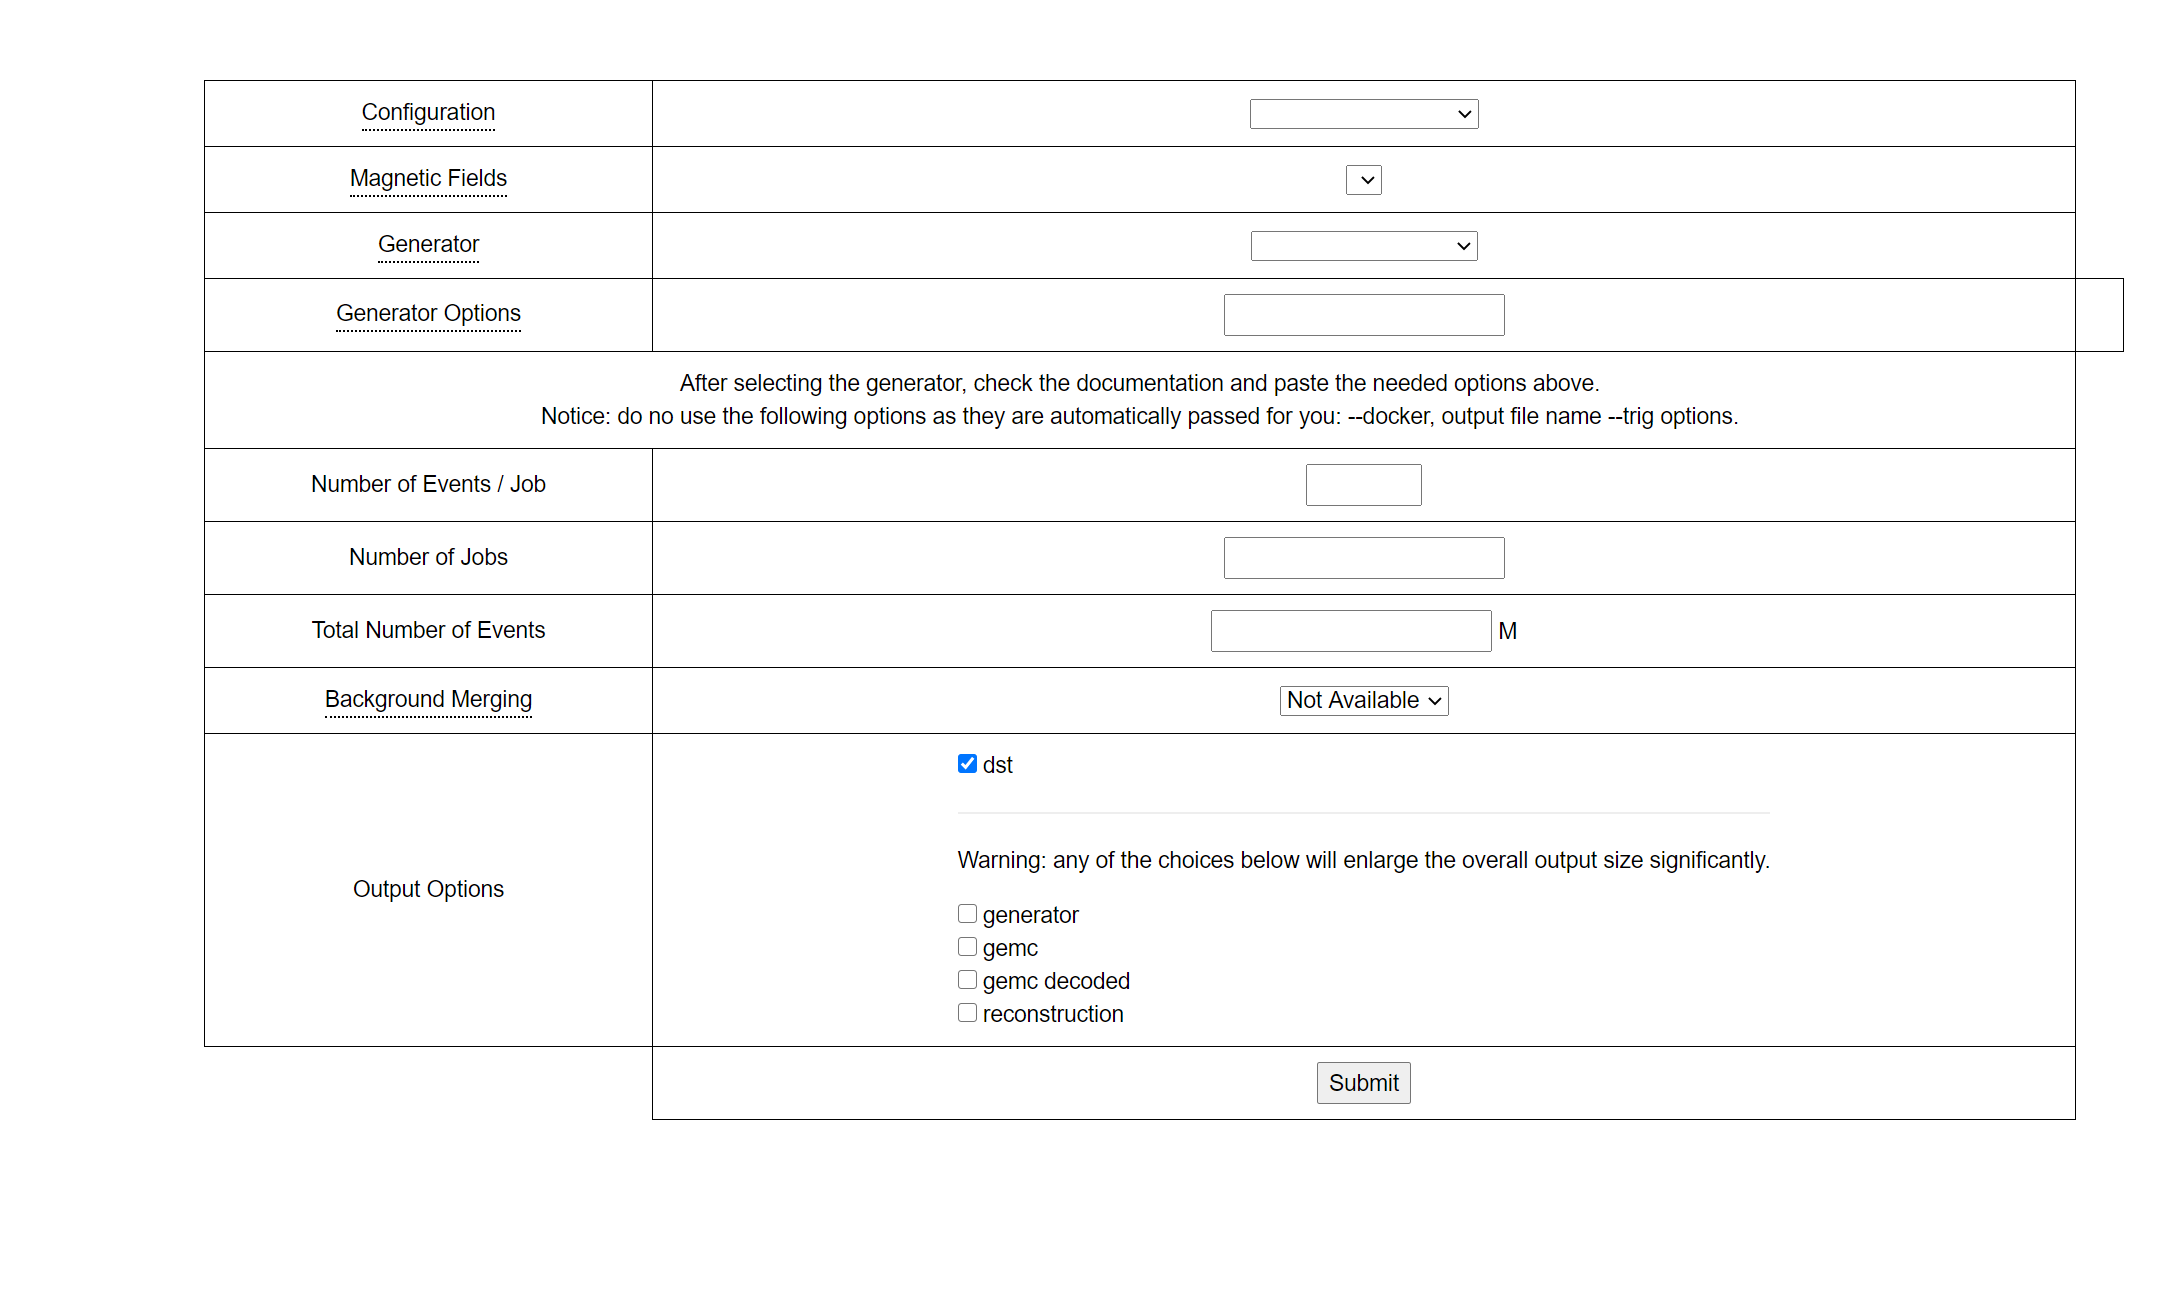
\includegraphics[width=16cm]{xxTasks/pics/pullthisin.png}
        \end{figure}


\section{Future Improvements}
    List of improvememnts that are not critical but might be nice in the future for someone who has time. Also these might be pushed up to more critical at any given time.
    \subsection{Include Priority}
        add priority to JSON (not to be used on normal production page, just the test page)
       SubMit/utils/update\_priority.py
    
       This is the way we handle priority P , which is basically P =  (constant) / N Running Jobs
    
    \subsection{Email Monitoring}
        If someone has the time, it is straightforward to set up triggers in python to send emails if things are broken. This would help in the case of system breaks. But, simulations do not usually run on ultra-critical time schedueles, so this is less important.
    \subsection{Live Generation and Usage of Container and Experiments}
        Generate in live-time on the webportal dependent quantities such as generator lists, configuration files, background merging file list 
    \subsection{Dynamic GCard Descriptions}
        Set up a dynamic list of gcards acceptable have list returned to user on what gcards are valid, can assume clas12.gcard \& a description of what gcard is / does / has in it
        Regarding the gcards, I think it's ok to have them in a file for now. We can wait a few container releases to see if what's in the file matches the container content or it has to be different. 
        The command to retrieve the list from the container is straightforward:
        
        \begin{lstlisting}
            singularity exec --home ${PWD}:/srv --pwd /srv --bind /cvmfs --contain --ipc --pid /cvmfs/singularity.opensciencegrid.org/jeffersonlab/clas12simulations:production ls /jlab/work/ | grep gcard
        \end{lstlisting}
        
    \subsection{Better Metrics / Logging}
        How will we log the number of events / the number of jobs if the user supplies the gcards / LUND files?
        use log output files to monitor job submissions

